\documentclass[10pt]{article}

\def\Type{LessonCaelan}
\def\TypeNum{Lesson 14}
\def\TypeTitle{Applied Optimization }
\def\Semester{Fall 2021} %Not Used 
\def\Course{MATH 1190 \& 1210}
\def\Targets{  {\bf\color{RedOrange}A3} }

\usepackage{preambleDJ}

%\usepackage{ragged2e}


%%%%%%%%%%%% BEGIN DOCUMENT %%%%%%%%%%%%%%%
%%%%%%%%%%%% BEGIN DOCUMENT %%%%%%%%%%%%%%%
%%%%%%%%%%%% BEGIN DOCUMENT %%%%%%%%%%%%%%%
%%%%%%%%%%%% BEGIN DOCUMENT %%%%%%%%%%%%%%%
%%%%%%%%%%%% BEGIN DOCUMENT %%%%%%%%%%%%%%%

\begin{document}

\pagestyle{otherpages}
\thispagestyle{firstpage}
\vs{.3}

\textbf{Intended Learning Outcomes}
After this lesson, you will be able to 

\begin{itemize}
    \item Define variables and translate assumptions with newly defined variables to model the applied context. (\target{A3})
    \item Convert given conditions (if any) into mathematical equations/expressions. (\target{A3})
    \item Set up objective function and convert it into a single-variable function (if needed). (\target{A3})
    \item Determine the domain of optimization based on the scenario. (\target{A3})
    \item Solve applied optimization problems. (\target{A3})
\end{itemize}

\vspace{-0.5cm}

\hrulefill\\

{\bf\color{blue}Read the Passage.} In the online pre-class activity, we saw optimization problems solved in two phases: the modeling phase and the calculus phase. We'll practice specific steps within each of those phases in this activity while re-attempting some of the same problems that appeared in the pre-class assignment - as well as while trying new problems.\\

Try to work through the following problem, which appeared in the pre-class assignment (with different numbers) as example 1. You don't have to get everything right - that you are willing to try something, figure out a method, and make some mistakes along the way is far more important than feeling pressured to get everything right the very first time.\\

{\bf\color{blue}Warm-up exercise 1.}\ltrm{\bf\color{RedOrange}A3} We want to build an open box (four side walls and a bottom but no top) with a square base. The volume of the box must be $256$ cm$^3$. We should build the box to spend as little on the materials as possible. What dimensions should we choose for our box?\\

\textbf{Modelling Phase:}\\
\mpageTth{.3}{.4}{.4}{
 \graphicsL{box}{2}
}{
$$SA=Bottom_{area}+Sides_{area}$$
}{
$$V=Length \times Width \times Height$$
}
\vs{1}~\\
\textbf{Calculus Phase:}

\vfill

%\end{document} %end here for written pre-class

%%%%%%%%%
\newpage%
%%%%%%%%%
{\bf Reflection: Modeling Phase} What steps did you take during the Modeling Phase? 
\vfill
{\bf Reflection: Calculus Phase} What steps did you take during the Calculus Phase? 
\vfill


\newpage

\begin{enumerate}

\LARGE \item We want to build a closed box with a square base. The volume of the box must be 256 cm$^3$. 

The top of the box costs $\$1$ per cm$^2$ of material, the sides of the box costs $\$0.50$ per cm$^2$ of material, and the bottom of the box costs $\$3$ per cm$^2$ of material. 

What dimensions should we choose for our box to minimize its cost?\\




%%%%%%%%%
\newpage%
%%%%%%%%%

\item Suppose the unit selling price of a commodity is $p(x)=4-\dfrac1{100}x$ and the total cost of producing a commodity is $C(x)=\dfrac{3}{100}x^2-6x+400$, with $0\leq x\leq 200$ for both.\\

Revenue is the income from the sales of a commodity. If $p(x)$ is the unit selling price of the $x^{th}$ unit of the commodity, then revenue from the sale of $x$ units of the commodity is: \[R(x)=x\cdot p(x)\]

Profit is the difference between revenue and total cost:
\[P(x) = R(x) - C(x)\]

How many units of the commodity should be sold to maximize profit?


\vfill


%%%%%%%%%
\newpage%
%%%%%%%%%

\item In economics, the actual cost incurred in producing an additional unit of a certain commodity at a certain level of operation is called the {\bf marginal cost}. Economists often define the marginal cost function to be the derivative of total cost. If the total cost of producing $x$ units of a product is $C(x)=x^2-4x^{3/2}+30$, then find the number of units to produce to minimize the marginal cost function.

%%%%%%%%%
\newpage%
%%%%%%%%%

\item A sheep farmer wishes to construct a rectangular pen enclosing 500 square feet partitioned into two pens using a fence parallel to one of the sides. (See the diagram below.) The fencing for the four outer sides of the pen must be heavy-duty (to keep out predators) and costs \$2 per foot. The interior (subdividing) fence costs \$1 per foot. What are the dimensions of the pen minimizing the cost?\\[0.1in]

\hspace{0.2in}
%
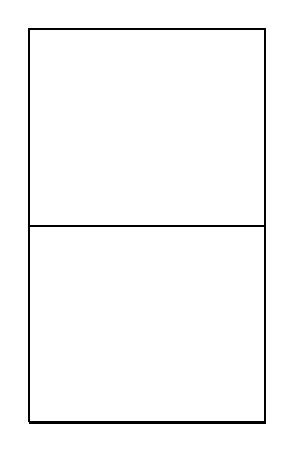
\begin{tikzpicture}
    \draw[thick] (0,0) -- (0,5) -- (3,5) -- (3,0) -- (0,0);
    \draw[thick] (0,2.5) -- (3,2.5);
\end{tikzpicture}



\newpage
\item A division of the Chapman Corporation manufactures a pager. The weekly fixed cost for the division is $\$20,000$ and the variable cost for producing $x$ pagers is $$V(x)=0.000001x^3-0.01x^2+50x$$ dollars. The company realizes a revenue of $$R(x)=-0.02x^2+150x \qquad (0\leq x \leq 7500)$$ from the sale of $x$ pagers per week. Find the level of production that will yield a maximum profit for the manufacturer.

%%%%%%%%%
\newpage%
%%%%%%%%%

\item A rectangular garden of area $40 ft^2$ is bounded on three sides by a fence costing \$2 per foot and on the 4th side by a fence costing \$1 per foot. 

Find the dimensions of this garden that will minimize the total cost.

%%%%%%%%%
\newpage%
%%%%%%%%%

\item A box with no top is to be constructed from a 20cm$\times$20cm sheet of cardboard by cutting four square pieces (in gray) of the same size from the corners of the sheet and then folding up the sides along the dotted lines.
 
 Find the side length of the gray square pieces to be cut that gives the largest volume of the box. 

\begin{figure}[h!]
\centering
 
\includegraphics[scale=0.6]{Fall 2025/Lessons/lesson14_AppliedOptimization/images/A4.png}
\end{figure}

%%%%%%%%%
\newpage%
%%%%%%%%%

\item Find two numbers differing by 48 whose product is as small as possible.

%%%%%%%%%
\newpage%
%%%%%%%%%

\item Owners of a car rental company have determined that if they charge customers $p$ dollars per day to rent a car, the number of cars $n$ they rent per day can be modeled by the linear function $n(p)=1000-5p$.

If they charge \$50 per day or less, they will rent all their cars. If they charge \$200 per day or more, they will not rent any cars. 

Assuming the owners plan to charge customers between \$50 per day and \$200 per day to rent a car, how much should they charge to maximize their revenue?

%%%%%%%%%
\newpage%
%%%%%%%%%

\item A rectangular box with a square base, an open top, and a volume of 216 cubic inches is to be constructed. 

What should the dimensions of the box be to minimize the surface area of the box?

\end{enumerate}

\end{document}
